\chapter{Anexo I: Matriz de Consistencia}


\begin{table}[h!]
	\centering
	\small
	\begin{tabular}{ |m{5cm}|m{5cm}|m{5cm}|  }
		\hline
		\rowcolor{bluejean}
		\Centering \color{white}{PROBLEMAS}& \Centering \color{white}{OBJETIVOS}& \Centering \color{white}{HIPÓTESIS}\\
		\hline
		\rowcolor{turq}
		\Centering Problema General& \Centering Objetivo General & \Centering Hipótesis General \\
		\hline
		{\ProblemaGeneral} & { \ObjetivoGeneral} & {\HipotesisGeneral} \\
		\hline
		\rowcolor{turq}
		\Centering Problemas Específicos& \Centering Objetivos Específicos & \Centering Hipótesis Específicas \\
		\hline
		{\Pbone} & {\Objone} & {\Hone} \\
		\hline
		{\Pbtwo} & {\Objtwo} & {\Htwo} \\
		\hline
		{\Pbthree} & {\Objthree} & {\Hthree} \\
		\hline
		{\Pbfour} & {\Objfour} & {\Hfour} \\
		\hline
	\end{tabular}
	\caption{Matriz de consistencia. Fuente: Elaboración propia}
	\label{1:table}
\end{table}



\chapter{Anexo II: Resumen de Papers investigados}
%\section{Conclusiones}

\begin{table}[h]
	\newcommand{\multirot}[1]{\multirow{2}{*}[-8ex]{\rotcell{\rlap{#1}}}}
	%\scriptsize
	\footnotesize
	\centering
	\begin{tabular}{|m{0.5cm}|m{0.3cm}|m{4cm}|m{2cm}|m{0.6cm}|m{1.7cm}|m{3cm}|} 
		\hline
		\rowcolor[rgb]{0,0.251,0.502} \multicolumn{1}{|c|}{\textcolor{white}{Tipo}} & \multicolumn{1}{c|}{\textcolor{white}{N°}} & \multicolumn{1}{c|}{\textcolor{white}{Título}}                                                                             & \multicolumn{1}{c|}{\textcolor{white}{Autor}}        & \multicolumn{1}{c|}{\textcolor{white}{Año}} & \multicolumn{1}{c|}{\textcolor{white}{País}} & \multicolumn{1}{c|}{\textcolor{white}{Fuente}}                                                        \\ 


		\hline
		\multirot{Problema}
		& 1         
		& Design and Development of AI-Powered Healthcare WhatsApp Chatbot
		& Prakasam S and N. Balakrishnan and Kirthickram T R and Ajith Jerom B and Deepak S
		& 2023
		& India
		& IEEE \\
		\cline{2-7}

		& 2        
		& Artificial Intelligence Powered Chatbot for Mental Healthcare based on Sentiment Analysis
		& Ansh Mehta and Sukhada Virkar and Jay Khatri and Rhutuja Thakur and Ashwini Dalvi
		& 2022
		& India
		& IEEE \\

		\hline
		\multirow{3}{*}[-14ex]{\rotcell{\rlap{Propuesta}}}
		& 3        
		& Use of chatbots for customer
		service in MSMEs
		& Jorge Cordero, Luis Barba-Guaman and Franco Guamán
		& 2022
		& Ecuador
		& Universidad Técnica Particular de Loja \\
		\cline{2-7}
		& 4        
		& Chatbot: una propuesta viable para la atención al cliente en el centro de soporte de la UCI
		& Rosbel Caballero Ramírez
		& 2021
		& Cuba
		& Revista Cubana de Ciencias Informática \\
		
		\hline
		\multirow{4}{*}[-28ex]{\rotcell{\rlap{Técnica}}}
		& 5        
		& The Science of Detecting LLM-Generated Text
		& Ruixiang Tang and Yu-Neng Chuang and Xia Hu
		& 2024
		& China
		& Communications of the ACM \\ 
		\cline{2-7}

		& 6        
		& Review on Implementation Techniques of 
		Chatbot
		& Nithuna S and Laseena C.A
		& 2020
		& India
		& International Conference on Communication and Signal Processing \\ 
		\cline{2-7}

		& 7        
		& AI-Based Chatbot
		& Aarush Saxena
		& 2024
		& India
		& International Journal for Research in Applied Science \& Engineering Technology (IJRASET) \\ 

		\cline{2-7}

		& 8        
		& Revisiting university students’ intention to accept AI-Powered chatbot with an integration between TAM and SCT: a south Asian perspective
		& Md. Rabiul Awal and Md. Enamul Haque
		& 2024
		& Bangladesh
		& ResearchGate - Journal of Applied Research in
		Higher Education \\ 
		\hline
	\end{tabular}
	\caption{Cuadro Resumen de Papers investigados. Fuente: Elaboración propia}
\label{A:table}
\end{table}


\chapter{Anexo III: Árbol del problema}

\begin{figure}[h]
	\begin{center}
		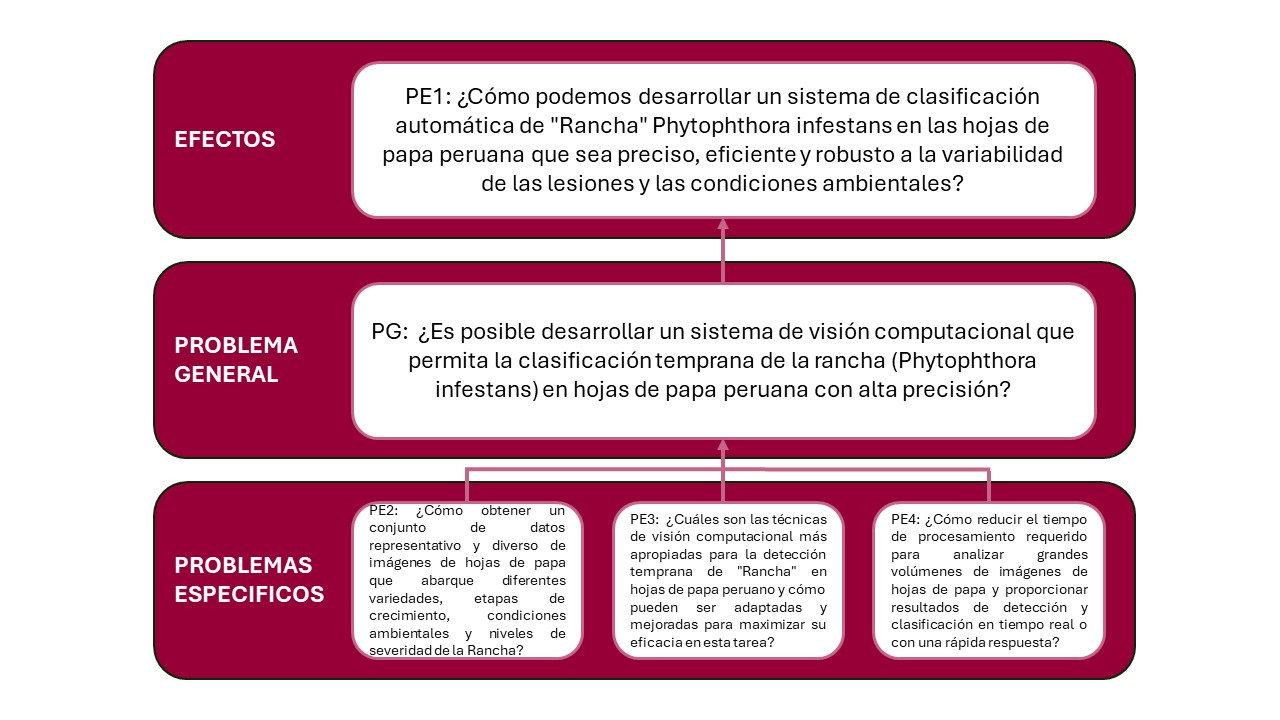
\includegraphics[width=0.75\textwidth]{anexos/arbol_problema.jpg}
		\caption{Arbol de problemas 
		\\Fuente: Creación Propia}
		\label{anexos:arbol_problema}
	\end{center}
\end{figure}

